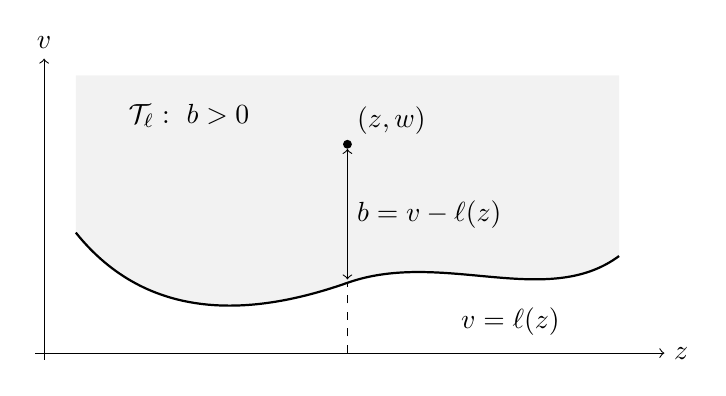
\begin{tikzpicture}[x=1.15cm,y=.85cm]
 \fill[black!5]
  (-3,1.8) .. controls (-2.2,.45) and (-1.05,.55) .. (0,1.05)
  .. controls (1.05,1.55) and (2.2,.65) .. (3,1.45)
  -- (3,4.15) -- (-3,4.15) -- cycle;
 \draw[->] (-3.45,0) -- (3.5,0) node[right] {$z$};
 \draw[->] (-3.35,-.1) -- (-3.35,4.4) node[above] {$v$};
 \draw[thick]
  (-3,1.8) .. controls (-2.2,.45) and (-1.05,.55) .. (0,1.05)
  .. controls (1.05,1.55) and (2.2,.65) .. (3,1.45);
 \node[anchor=north] at (1.8,.82) {$v=\ell(z)$};
 \draw[dashed] (0,0) -- (0,1.05);
 \draw[<->] (0,1.1) -- (0,3.05)
  node[midway,right] {$b=v-\ell(z)$};
 \fill (0,3.12) circle (1.6pt);
 \node[above right] at (0,3.12) {$(z,w)$};
 \node at (-1.75,3.55) {$\mathcal T_\ell:\ b>0$};
\end{tikzpicture}
